% !TEX program = pdflatex
% !BIB program = biber
% !TeX spellcheck = en_US
% !TeX encoding = UTF-8
% !TeX root = main.tex

%%%%%%%%%%%%%%%%%%%%%%%%%%%%%%%%%%%%%%%%%
% University of St.Gallen
% Interaction- and Communication-based Systems
% https://interactions.ics.unisg.ch/
%
% LaTeX Template
% Version 0.1 (21.05.2021) Iori Mizutani
%%%%%%%%%%%%%%%%%%%%%%%%%%%%%%%%%%%%%%%%%
%----------------------------------------------------------------------------------------
%	PACKAGES AND OTHER DOCUMENT CONFIGURATIONS
%----------------------------------------------------------------------------------------
\documentclass[a4paper,11pt]{article}
\usepackage[english]{babel}
\usepackage[utf8]{inputenc}
\usepackage{amsmath}
\usepackage{amssymb}
\usepackage{amsfonts}
\usepackage[backend=biber]{biblatex}
\addbibresource{bibliography.bib}
% Allow long URLs in the bibliography to break across lines.
\setcounter{biburllcpenalty}{7000}
\setcounter{biburlucpenalty}{8000}
% Last-resort stretch for lines with no good break point (long titles, URLs).
\setlength{\emergencystretch}{1em}
\usepackage{graphicx}
\usepackage[toc,page]{appendix}
\usepackage{geometry}
\geometry{
 a4paper,
 total={170mm,257mm},
 left=20mm,
 top=20mm,
}
\usepackage{xcolor}
\usepackage{hyperref}
\usepackage{tikz}
\usetikzlibrary{shapes.symbols,calc}
\usepackage{ctable}
\usepackage{url}
\usepackage{titling}

\author{Jahrim Gabriele Cesario}
% \title carries the line break for the title page; PDF metadata needs a plain
% single-line string, since \thetitle reaches \pdftitle already expanded.
\newcommand{\titleplain}{Semantic-Aware Foundations for Theorem Proving}
\title{Semantic-Aware Foundations\\for Theorem Proving}


\hypersetup{
    unicode=false,          % non-Latin characters in Acrobat’s bookmarks
    pdffitwindow=true,      % window fit to page when opened
    pdfstartview={FitH},    % fits the width of the page to the window
    pdftitle={\titleplain}, % title
    pdfauthor={\theauthor}, % author
    colorlinks=false,       % false: boxed links; true: colored links
    linkbordercolor=red,    % color of internal links (change box color with linkbordercolor)
    citebordercolor=green,  % color of links to bibliography
    filebordercolor=magenta,% color of file links
    urlbordercolor=cyan     % color of external links
}

% \system takes an optional font command (default: italic). The line-broken
% variant is separate: a \\ must stay outside the font group to remain a line
% break inside a TikZ node.
\NewDocumentCommand{\system}{O{\textit}}{#1{Smart E-Graphs}}
\newcommand{\systemstacked}{Smart\\E-Graphs}

\begin{document}
\begin{titlepage}

 % Defines a new command for the horizontal lines, change thickness here
\newcommand{\HRule}{\rule{\linewidth}{0.5mm}}
\setlength{\topmargin}{0in}
 % Center everything on the page
\center
\includegraphics[height=1.5cm]{logos/hsg.pdf}
\hfill
\includegraphics[height=1.3cm,trim=0 4mm 0 4mm]{logos/prg-grp.pdf}

%----------------------------------------------------------------------------------------
%	HEADING SECTIONS
%----------------------------------------------------------------------------------------

\vfill
\textsc{\Large Ph.D. in Computer Science (DCS)} \\[0.5cm]
\textsc{\LARGE University of St.Gallen}\\[2.0cm]

%----------------------------------------------------------------------------------------
%	TITLE SECTION
%----------------------------------------------------------------------------------------

\HRule \\[0.6cm]
% Title of your document
\huge \textbf{\thetitle}\\[0.4cm]
\HRule \\[0.4cm]

\textsc{\Large Research Proposal}
\vfill

%----------------------------------------------------------------------------------------
%	AUTHOR SECTION
%----------------------------------------------------------------------------------------

\begin{minipage}{0.4\textwidth}
\begin{flushleft} \large
\emph{PhD Student:}\\
% Your name
\theauthor \\ 
\end{flushleft}
\end{minipage}
~
\begin{minipage}{0.5\textwidth}
\begin{flushright} \large
\emph{Advisor:} \\
Prof. Dr. Guido \textsc{Salvaneschi} \\
Institute of Computer Science\\
University of St.Gallen\\[0.5cm]
\emph{Co-Advisor(s):} \\
Prof. Dr. Max \textsc{Willsey}\\
Department of Electrical Engineering and Computer Sciences\\
University of California, Berkeley
%\emph{Other Supervisors} \\
% \textsc{Add name here} % Supervisor's Name
% Supervisor Department(s) or NHS Trust+section
\end{flushright}
\end{minipage}\\[2cm]

%----------------------------------------------------------------------------------------
%	DATE SECTION
%----------------------------------------------------------------------------------------

% Date, change the \today to a set date if you want to be precise
{\large \today}

\vfill % Fill the rest of the page with whitespace

\end{titlepage}

% !TeX spellcheck = en_US
% !TeX encoding = UTF-8
% !TeX root = main.tex

\section*{Abstract}

Software verification is the discipline of establishing that a program meets its
specification and is indispensable to improve our understanding of software 
systems and ensure their reliability. 
Theorem proving pursues verification by constructing formal machine-checkable 
proofs of correctness, in a logic that can capture program semantics.
Constructing such proofs turns repeatedly on deciding whether terms are equal,
and many theorem provers rest on a common foundation for equational reasoning.
Reasoning in verification, however, is rarely about equality alone. 
Proofs split into cases, argue under assumptions, and appeal to facts that hold 
only conditionally, but provers today capture this richer semantics around that 
foundation rather than within it. This proposal argues that the foundation
itself should reason beyond equality, letting provers do more of their work at
the level they already share.

We pursue this idea for the e-graph, the equality-reasoning data structure at 
the heart of many provers. Our project, \system, moves that richer semantics
inside the e-graph: disequalities and conditional facts become part of the
structure itself, and provers reason about them natively. These semantic
extensions open room for optimizations, since one enriched structure can reuse
work that separate encodings would repeat, and because the e-graph underlies so
many provers, these gains extend well beyond any single tool. We plan to realize our
idea in a single artifact that integrates with existing provers and, through
them, reaches the broader verification ecosystem.

\newpage

\section{Introduction}



\begin{figure}[t]
    \centering
    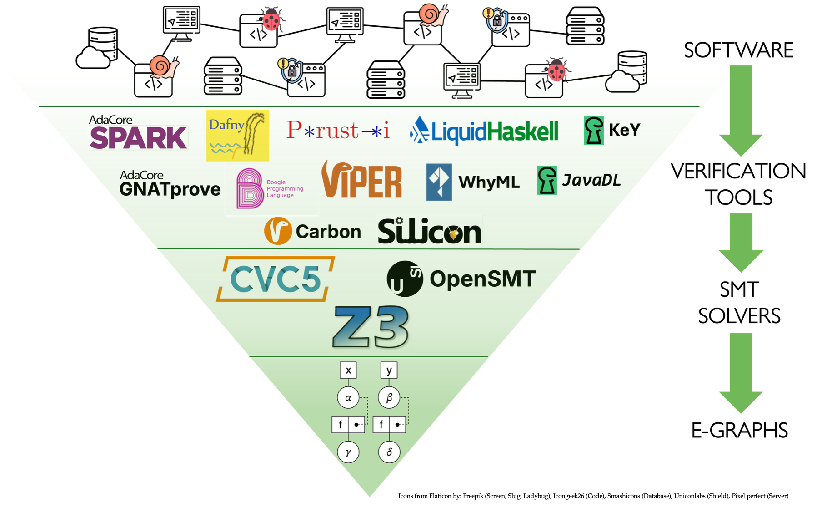
\includegraphics[width=0.7\textwidth]{figures/pyramid.pdf}
    \caption{The static verification ecosystem based on SMT solvers and e-graphs.}
\end{figure}

\textit{Software verification} is the discipline of assuring that a software system
conforms to a given specification. It is a traditional area of research in 
computer science, drawing on both \textit{software engineering} and 
\textit{programming languages}.
\textit{Dynamic verification}, such as \textit{testing} and \textit{fuzzing}, 
executes the system under selected configurations to discover deviations from 
the specification, i.e., \textit{bugs}. 
Instead, \textit{static verification}, such as \textit{model checking} and
\textit{theorem proving}, analyzes all possible system's behaviors to guarantee 
that it always satisfies the specification. Since this is rarely feasible for 
complex systems, static verification often relies on
\textit{abstractions} that approximate the system and the specification to make
the analysis tractable. In that sense, it is \textit{static} because the 
analysis is performed without executing the original system.

In this proposal, we focus on \textit{static verification} and specifically on
\textit{theorem proving} for software verification.


\paragraph{What is verification?} The process of guaranteeing that a system
satisfies a specification\dots

\paragraph{Why is it significant?} Soundness guarantees compared to testing,
formal methods for AI, \dots

\paragraph{What are the verification tools?} SMT solvers, saturation-based, eqsat-based, Lean, Coq, Isabelle, Agda, \dots

\paragraph{What are the challenges?} Scalability, usability, \dots

\paragraph{What is the contribution of this PhD proposal?} Optimizing the
verification ecosystem based on e-graphs \dots

\paragraph{What is the impact?} Proving more and faster \dots


\section{Background}

This section reviews the background that motivates our proposal and the prior
work it builds on. We begin with the landscape of theorem provers, identifying
which of them stand to benefit from our contributions, and then describe the
data structures that will be extended.

\subsection{Theorem Provers}

\paragraph{Automated Theorem Provers.}
\textit{Automated theorem provers} discharge goals without human guidance, and how
much each stands to gain from our work depends on how centrally it relies on
e-graphs. \textit{SMT solvers} such as Z3~\cite{demoura2008z3} and
cvc5~\cite{barbosa2022cvc5} use congruence closure and e-matching as a core
theory solver, so extensions to the e-graph reach them directly.
\textit{Verification languages} such as Dafny~\cite{leino2010dafny},
Viper~\cite{mueller2016viper}, and F*~\cite{swamy2016fstar} compile programs and
their specifications to SMT queries, and so benefit indirectly, through their
solver backend. \textit{Equality-saturation} tools, including
egg~\cite{willsey2021egg} and the inductive provers TheSy~\cite{singher2021thesy}
and CCLemma~\cite{kurashige2024cclemma}, make the e-graph the central
representation for exploring rewrites, and stand to gain the most. By contrast,
\textit{saturation-based} superposition provers such as
Vampire~\cite{kovacs2013vampire} and E~\cite{schulz2013e} organize their search
around term indexing and ordered rewriting rather than a shared e-graph, and are
the least likely to benefit from this line of work.

\paragraph{Interactive Theorem Provers.}
\textit{Interactive theorem provers} let a user steer the proof while the tool
checks each step. Their kernels rest on rich type theories or higher-order
logics, as in Isabelle~\cite{nipkow2002isabelle}, Coq~\cite{bertot2004coq},
Agda~\cite{norell2009agda}, and Lean~\cite{demoura2021lean4}, and this core
proof checking does not use e-graphs, so our extensions have little to offer it.
Their proof automation is another matter: e-graph-based tactics such as Lean's
\texttt{grind}~\cite{leangrind} and Coq's congruence closure~\cite{corbineau2007congruence}
discharge goals by saturating an e-graph with the available facts, and it is
these components, rather than the kernels, that our work stands to improve.

\subsection{Equational Reasoning}

\paragraph{Union-Find.}
A \textit{union-find}, or disjoint-set structure~\cite{tarjan1975union},
maintains an \textit{equivalence relation} over a set of elements using two
operations: \textit{find} returns a canonical representative of the class
containing an element, so that two elements are equivalent exactly when they
share a representative, and \textit{union} merges two classes by making one
representative point to the other. With union by rank and path compression, both
run in near-constant amortized time~\cite{tarjan1984worstcase}. The structure
thus maintains precisely the equivalence relation generated by the equalities
asserted so far, that is, their reflexive, symmetric, and transitive closure, but
records nothing about the structure of the terms that name the elements.

\paragraph{E-Graphs.}
An \textit{e-graph}~\cite{nelson1980congruence, willsey2021egg} lifts this idea
from opaque elements to functional \textit{terms}, maintaining not merely an equivalence
relation but a \textit{congruent} one: a relation additionally closed under
congruence, so that whenever the arguments of a function are pairwise
equivalent, the applications are too. A term is stored as an \textit{e-node}, a
function symbol applied to a tuple of child \textit{e-classes}, and an e-class is
a set of e-nodes that have been proven equal. Internally, an e-graph is a
union-find over e-class identifiers together with a hash-cons mapping each e-node
to its e-class, so \textit{find} and \textit{union} carry over unchanged.
Merging two e-classes with \textit{union}, however, can break the congruence
invariant, since two e-nodes that have just become congruent may still sit in
different e-classes. For example, suppose an e-graph holds the terms $f(a)$ and
$f(b)$ in distinct e-classes; asserting $a = b$ merges the classes of $a$ and
$b$, so congruence now demands $f(a) = f(b)$, yet the two applications still sit
in separate e-classes until the invariant is restored. The \textit{rebuild}
operation restores the invariant by
repeatedly merging such newly congruent e-nodes until a fixpoint is
reached~\cite{willsey2021egg}. An e-graph therefore represents the
\textit{congruent equivalence relation} generated by the asserted equalities,
that is, their reflexive, symmetric, transitive, and congruent
closure~\cite{zakhour2025disequality}.

\paragraph{Equality Saturation.} \textit{Equality saturation}~\cite{tate2009eqsat, willsey2021egg}
is a framework built around e-graphs that repeatedly applies a set of rewrite 
rules, non-destructively so that
rules need not be ordered, until it is \textit{saturated} or a resource bound is
reached. Then, one can \textit{extract} an optimal representative under a cost
model or prove two terms equal under the axioms of the rewrite rules. In detail,
each rewrite $\ell \to r$ is applied by \textit{e-matching}, finding all
instances of the pattern $\ell$ up to the equivalences the e-graph
records~\cite{demoura2007ematching} and making $r$ equal to every match.
Sidestepping the \textit{phase-ordering} problem this way, equality saturation
underlies applications from compiler optimization~\cite{tate2009eqsat} to
inductive theorem proving, as in TheSy~\cite{singher2021thesy} and
CCLemma~\cite{kurashige2024cclemma}, while the same e-matching mechanism drives
quantifier instantiation in SMT solvers~\cite{demoura2007ematching}.

\section{Course Phase}

\subsection{Survey of related work.} literature review \dots

\subsection{Disequality Reasoning.} contribution \dots

\subsection{Conditional Reasoning.} authored \dots

\section{Dissertation Phase}

\subsection{Lazy Reasoning}

\paragraph{Lazy Operations} e.g., union and intersection of e-graphs \dots

\subsection{Parallel Reasoning} 

\paragraph{Lattice of E-Graphs} how to define dependencies between proof
exploration tasks in terms of e-graphs\dots

\paragraph{Static Scheduling} how to schedule proof exploration tasks in 
parallel on a complete lattice\dots

\paragraph{Dynamic Scheduling} how to schedule proof exploration tasks in
parallel on a partial lattice (some information are missing)\dots

\subsection{Integration with Verification Tools}

\paragraph{Integration with SMT solvers} e.g., Z3 \dots

%**********************************************%
\printbibliography

\end{document}
